ในส่วนของงานวิจัยนี้สิ่งที่สนใจ คือ ข้อมูลการกระทำของมนุษย์แต่ละคนภายในวิดีโอ เพื่อที่จะได้ผลลัพธ์ที่มีประสิทธิภาพออกมาเป็นข้อมูลของสิ่งที่สนใจ เช่น จำนวนคนที่เดินผ่านกล้อง 
หรือทิศทางการเดินของคนในวิดีโอ จึงจำเป็นต้องใช้การประมวลผลวิดีโอเพื่อที่จะสกัดสิ่งที่สนใจออกมาจากวิดีโอ ซึ่งการประมวลผลวิดีโอมีหลากหลายกระบวนการ 
โดยในแต่ละกระบวนการจะมีจุดประสงค์ของการทำและผลลัพธ์หลังการประมวลผลที่แตกต่างกัน ในหัวข้อนี้จะมาอธิบายถึงกระบวนการในการประมวลผลของวิดีโอและผลลัพธ์ของกระบวนการนั้น
\subsection{การตรวจจับวัตถุ}
การตรวจจับวัตถุนั้นเป็นหนึ่งในกระบวนการประมวลผลวิดีโอ\textsuperscript{\cite{object_detection}} กล่าวคือกระบวนการที่ผู้วิจัยจะต้องทำการระบุสิ่งที่สนใจว่า คืออะไร อยู่ที่ตำแหน่งใด การตรวจจับวัตถุถูกค้นพบเป็นเวลานานมาแล้ว 
และในปัจจุบันนั้นสามารถทำได้หลากหลายวิธี โดยภายในบทความนี้จะสรุปใจความสำคัญของวิธีการต่างในการตรวจจับวัตถุ เช่น Sliding window, Brute force search, RCNN, 
Fast-RCNN, Faster-RCNN, YOLO, SSD 
\begin{enumerate}
	\item Sliding window วิธีการที่เปรียบเสมือนมีเคอร์เนลค่อยๆเลื่อนไปยังแต่ละพิกเซลบนภาพ ซึ่งก่อนการเลื่อนของเคอร์เนลแต่ละครั้งจะนำส่วนของภาพที่ถูกเคอร์เนลทับอยู่ไปทำนายว่าใช่วัตถุที่เราต้องการหรือไม่ 
	จากนั้นจึงค่อยเลื่อนถัดไปจนครบทั้งภาพ
	\item Brute force search ถูกสร้างขึ้นมาเพื่อแก้ปัญหาขนาดของเคอร์เนลไม่ตรงกับขนาดของวัตถุที่อยู่ในภาพทำให้มีโอกาสที่จะไม่พบวัตถุ โดยหลักการของวิธีการนี้คือ 
	การย่อ-ขยายภาพและนำเข้าในหลายๆอัตราส่วน ตั้งแต่ 0.1 เท่า จนถึง 2 เท่า แต่ข้อเสียของวิธีการนี้คือ มีการคำนวณพื้นที่ซ้ำๆทำให้ใช้เวลานาน
	\item RCNN ใช้อัลกอริทึม selective search เข้ามาช่วยในการหาพื้นที่ที่น่าจะมีวัตถุอยู่ทดแทนการค้นหาทุกๆตำแหน่ง จากนั้นก็นำภาพในส่วนพื้นที่นั้นไปทำนายว่าวัตถุนั้นคืออะไร 
	กรณีที่มีพื้นที่ที่อยู่ใกล้ๆวัตถุถูกเสนอเข้ามาเป็นจำนวนมากด้วย เราจะใช้ NMS ในการเลือกพื้นที่ที่ถูกทับซ้อนมากที่สุดในบริเวณนั้น
	\item Fast-RCNN จากวิธีการ RCNN แต่ละพื้นที่จะถูกนำไปสกัดคุณลักษณะ และทำนายผลทีละพื้นที่ทำให้เสียเวลา โดย Faster-RCNN จะมีส่วนที่คล้ายกับ RCNN ในส่วนการทำ 
	selective search เพื่อหาพื้นที่ที่น่าจะมีวัตถุเหมือนเดิม แต่ Faster-RCNN จะนำภาพไปสกัดคุณลักษณะ หลังจากที่ได้คุณลักษณะแล้วจะนำพิกัดของพื้นที่ที่น่าจะมีวัตถุ 
	บนภาพที่ถูกสกัดคุณลักษณะแล้วไปผ่านชั้น ROI Pooling (การลดขนาดข้อมูลให้มีขนาดคงที่เพื่อเป็นข้อมูลป้อนเข้าให้กับโมเดลในการทำนายผล)
	\item Faster-RCNN พัฒนาจาก Fast-RCNN โดยวิธีของ Faster-RCNN จะรวมในส่วนของ selective search และการทำงานอื่นๆให้อยู่ในโครงข่ายเดียวกัน 
	สรุปคือการทำงานของโครงข่ายของ Faster-RCNN จะมีการทำงานสามอย่างคือ 1) สกัดคุณลักษณะ 2) การหาส่วนที่น่าจะมีวัตถุอยู่ในภาพ 3) หลังจากได้ภาพจากการสกัดคุณลักษณะ 
	นำพิกัดของพื้นที่ที่น่าจะมีวัตถุบนภาพที่ถูกสกัดคุณลักษณะแล้วไปผ่านชั้น ROI Pooling
	\item YOLO เป็นวิธีการที่ใช้ CNN เพียงตัวเดียวทำนายภาพ โดยโครงข่ายจะแบ่งภาพออกเป็นพื้นที่ และใช้ fully connected การติดตามการเคลื่อนไหวตำแหน่งของกรอบสี่เหลี่ยม 
	พร้อมทั้งหมวดหมู่ของวัตถุไปพร้อมกัน 
	\item SSD ใช้โครงข่ายประสาทเทียมเหมือนกับ YOLO แต่การออกแบบโครงสร้างแตกต่างกัน โดยที่ SSD จะใช้ VGG-16 ในการสกัดคุณลักษณะ และใช้ Convolution layer 
	ต่อกันหลายๆชั้นเพื่อลดมิติและความละเอียดทำให้ตรวจจับวัตถุในหลายๆขนาด ซึ่งในแต่ละชั้นจะได้ผลออกมาเป็น Convolution filter จากนั้นจะนำ Convolution filter ไปทำนายผลต่อ
\end{enumerate}

\subsection{การติดตามการเคลื่อนไหวของวัตถุ}
การติดตามการเคลื่อนไหวของวัตถุ\textsuperscript{\cite{danelljan2014accurate}} คือระบบที่ใช้สำหรับการติดตามการเคลื่อนไหวของวัตถุที่สนใจที่อยู่ในรูปภาพ 
โดยใช้การคำนวณทางคณิตศาสตร์ และการประมวลผลภาพ (image processing) ทำให้การประมวลผลนั้นเร็วกว่าการใช้โมเดลปัญญาประดิษฐ์ ซึ่งอัลกอริทึมติดตามการเคลื่อนไหวที่นิยมใช้มีสองอัลกอริทึม
คือ correlation filter และ kalman filter ซึ่งหลักการของทั้งสองอัลกอริทึมนั้นจะแตกต่างกันโดยที่ correlation filter นั้นจะใช้พิกเซลของวัตถุในการคำนวณตำแหน่งถัดไปของวัตถุ 
และ kalman filter จะใช้ข้อมูลการเคลื่อนไหวในการคำนวณตำแหน่งถัดไปของวัตถุ ซึ่งจากการศึกษาในบทความ "Object Tracking using Correlation,
Kalman Filterand Fast Means Shift Algorithms"\textsuperscript{\cite{ali2006object}} kalman filter มีประสิทธิภาพที่สูงนั้นจะขึ้นอยู่กับข้อมูลที่ได้จากการวัด (measurement)
และความซับซ้อนในการเคลื่อนไหวของวัตถุ ในขณะที่ correlation นั้นมีประสิทธิภาพที่ด้อยกว่า kalman filter เพียงเล็กน้อยและสามารถติดตามการเคลื่อนไหวที่ซับซ้อนของวัตถุได้ดีกว่า 
(การเคลื่อนไหวที่ซับซ้อนหมายถึง การเคลื่อนไหวที่เกิดการเปลี่ยนทิศทางฉับพลันบ่อย) ผู้วิจัยจึงตัดสินใจเลือกใช้ correlation filter ในงานครั้งนี้
\begin{figure}[!ht]
	\centering
	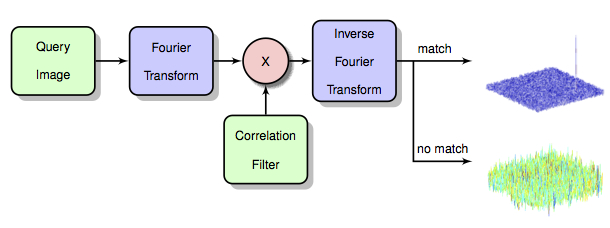
\includegraphics[width=1\textwidth]{chapter2/images/track-concept.png}
		\caption[แนวคิดของระบบติดตามการเคลื่อนไหวของวัตถุ]{แนวคิดของระบบติดตามการเคลื่อนไหวของวัตถุ\textsuperscript{\cite{correlation_filter}}}
    	\label{fig:Track_concept}
\end{figure}

จากรูปที่ \ref{fig:Track_concept} เป็นหลักการในการติดตามการเคลื่อนไหวของวัตถุแบบ correlation filter โดยการนำรูปมาผ่านกระบวนการแปลงฟูรีเยร์ (fourier transform)
และนำมาคูณกับ correlation filter ซึ่งเป็นตัวกรองที่ใช้สำหรับการหาความสัมพันธ์กับวัตถุในภาพ จากนั้นทำการแปลงฟูรีเยร์ผกผัน (inverse fourier transform) 
เพื่อตรวจสอบว่าวัตถุในภาพนั้นอยู่ที่ตำแหน่งใด โดยมีการคำนวณเริ่มจากการหา correlation filter ที่ดีที่สุดโดยใช้วิธีลดผลรวมของข้อผิดพลาดกำลังสองให้น้อยที่สุดดังนี้

\begin{equation}
\epsilon = \left \| \sum_{l = 1}^{d} h^{l} \star f^{l} - g \right \|^2 + \lambda \sum_{l = 1}^{d}\left \| h^{l} \right \|^2
\end{equation}
โดยที่
\begin{conditions}
 \epsilon     	&   ค่าความคลาดเคลื่อน 							\\
 d      		&  จำนวนมิติของผังคุณลักษณะของภาพ  \\   
 h 			&  correlation filter								\\
\star 			&  circular correlation							\\
 f			&  พื้นที่สี่เหลี่ยมของวัตถุที่สนใจที่ได้จากการทำผังคุณลักษณะ	\\
 g			&  ผลลัพธ์ correlation ที่ต้องการของ f					\\
 \lambda   		&  regularization term
\end{conditions}

เมื่อพิจารณาจากรูปภาพเดียวในกรณีที่เวลา ($t$) เท่ากับ 1 จะสามารถจัดรูปสมการด้านบนได้ดังนี้ 

\begin{equation}
H^{l} = \frac{\bar{G}F^{l}}{\sum_{k=1}^{d}\bar{F^{k}}F^{k} + \lambda}
\end{equation}
\begin{equation}
H_{t}^{l} = \frac{A_{t}^{l}}{B_{t}}					
\end{equation}					
\begin{equation}
A_{t}^{l} = (1-\eta )A_{t-1}^{l} + \eta \bar{G_{t}}F_{t}^{l}
\end{equation}
\begin{equation}
B_{t} = (1-\eta )B_{t-1} + \eta \sum_{k=1}^{d}\bar{F_{t}^{k}}F_{t}^{k}
\end{equation}
\clearpage
\noindent
โดยที่
\begin{conditions}
 H 		     	&   correlation filter								\\
 \eta      		&  อัตราการเรียนรู้						 		\\   
 \bar{G} 		&  g ที่ผ่านการทำ complex conjugation					\\
 F			&  พื้นที่สี่เหลี่ยมของวัตถุที่สนใจที่ได้จากการทำผังคุณลักษณะ	\\
 \bar{F}		&   f ที่ผ่านการทำ complex conjugation					\\
 t 	  		&  เวลา
\end{conditions}
จากสมการที่ได้มาจะสามารถทำให้หาตำแหน่งต่อไปของวัตถุที่สนใจได้ด้วยสมการต่อไปนี้
\begin{equation}
y = F^{-1}\left \{ \frac{\sum_{l = 1}^{d} \bar{A^{l}}Z^{l}}{B + \lambda} \right \}
\end{equation}
โดยที่
\begin{conditions}
 y 		     	&   correlation score										\\
 F^{-1}    		&  การแปลงฟูรีเยร์ผกผันแบบไม่ต่อเนื่อง (inverse discrete fourier transform)						\\   	
 \bar{A}^{l} 	&  $A^{l}$ ที่ผ่านการทำ complex conjugation				\\
 Z	 		&  พื้นที่สี่เหลี่ยมของวัตถุที่สนใจที่ได้จากการหาผังคุณลักษณะของภาพใหม่	
\end{conditions}
โดยค่าของ $y$ ที่ได้ออกมาจะทำให้รู้ถึงตำแหน่งของวัตถุที่สนใจได้ ณ ตำแหน่งที่ $y$ มีค่าสูงสุด

\clearpage
\subsection{การระบุตัวตนของบุคคล}
ระบบระบุตัวตนของบุคคล\textsuperscript{\cite{luo2019alignedreid++}}\textsuperscript{\cite{zhang2017alignedreid}} คือการระบุตัวตนของบุคคลภายในวิดีโอหรือระหว่างสองภาพ สามารถนำมาประยุกต์ใช้ในด้านของการรักษาความปลอดภัย 
หรือการตามหาบุคคล ซึ่งการระบุตัวตนของบุคคลนั้นเป็นปัญหาที่ท้าทาย เนื่องจากคุณลักษณะทั่วไปของบุคคลในภาพไม่เพียงพอต่อการระบุตัวตนภายในภาพว่าเป็นบุคคลคนเดียวกันได้ ซึ่งวิธีการที่ใช้ในการระบุตัวตนของบุคคลเรียกว่า 
Dynamically Matching Local Information (DMLI) ที่สามารถจัดแนวรายละเอียดข้อมูลของภาพและเพิ่มประสิทธิภาพให้สูงขึ้น 
ถึงแม้ว่า DMLI นั้นจะไม่ใช่วิธีการที่มีประสิทธิภาพสูงสุดแต่มีประสิทธิภาพใกล้เคียงกับโมเดลอื่นๆ แต่ผู้วิจัยสามารถนำวิธีนี้มาประยุกต์เข้ากับงานวิจัยครั้งนี้ได้สะดวกที่สุด จึงนำวิธีการนี้มาใช้สำหรับงานวิจัยครั้งนี้

\begin{figure}[!ht]
	\centering
	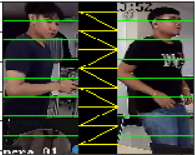
\includegraphics[width=0.3\textwidth]{chapter2/images/alignedreid.png}
		\caption{การแบ่งภาพออกเป็น 8 ส่วนของระบบระบุตัวตนของบุคคล}
    	\label{fig:alignedreid}
\end{figure}

การทำงานของระบบระบุตัวตนของบุคคลจะเริ่มจากการแบ่งภาพออกเป็น 8 ส่วนและนำคุณลักษณะทั่วไปของภาพมาผ่านกระบวนการ normalization เพื่อลดความซ้ำซ้อนของข้อมูล 
แล้วนำมาเปรียบเทียบความแตกต่างของคุณลักษณะทั่วไปของภาพโดยใช้วิธี euclidean distance หลังจากนั้นใช้วิธี DMLI หาความแตกต่างออกมา โดยค่าที่ได้ออกมาจะเรียกว่า aligned distance ถ้าค่าที่ออกมาใกล้เคียงกับศูนย์
จะหมายถึงบุคคลในภาพทั้งสองเป็นบุคคลเดียวกัน โดยใช้การกำหนดเกณฑ์ของ aligned distance สำหรับระบุตัวตนของบุคคลในภาพว่าเป็นบุคคลเดียวกันหรือไม่

โดยชุดข้อมูลที่นำมาใช้สำหรับการทำโมเดลปัญญาประดิษฐ์ได้แก่
\begin{enumerate}
	\item{Market1501 เป็นชุดข้อมูลที่เก็บข้อมูลภาพของบุคคลโดยใช้กล้องจำนวนหกตัว ถ่ายภาพบุคคลที่ด้านหน้าของซุปเปอร์มาร์เก็ตในมหาวิทยาลัย Tsinghua}
	\item{DukeMTMCReID เป็นชุดข้อมูลที่เก็บข้อมูลภาพของบุคคลโดยใช้กล้องจำนวนแปดตัว ถ่ายภาพบุคคลที่วิทยาเขตของมหาวิทยาลัย Duke ซึ่งมีการเก็บภาพมากถึงสองล้านภาพของนักศึกษาสองพันคน }
	\item{CUHK-03 เป็นชุดข้อมูลที่เก็บภาพของบุคคลที่มหาวิทยาลัยที่ฮ่องกง}
	\item{MSMT17 เป็นชุดข้อมูลที่เก็บข้อมูลภาพของบุคคลโดยใช้กล้องจำนวนสิบห้าตัว โดยที่กล้องแต่ละตัวจะไม่ได้ตั้งอยู่สถานที่เดียวกัน และเก็บข้อมูลที่ในวันที่มีสภาพอากาศต่างกัน}
\end{enumerate}

โดยทุกชุดข้อมูลจะใช้โครงสร้าง (architecture) ResNet50 ในการสร้างโมเดลปัญญาประดิษฐ์ และทดสอบด้วยวิธี Global+DMLI คือการนำคุณลักษณะทั่วไปและคุณลักษณะจำเพาะของภาพที่ได้มาจากโมเดลปัญญาประดิษฐ์ นำมาหาค่าระยะความแตกต่าง โดยที่ค่าระยะความแตกต่างของคุณลักษณะทั่วไปสามาหาได้โดยใช้วิธี Euclidean distance และค่าระยะความแตกต่างของคุณลักษณะจำเพาะสามารถหาได้โดยใช้วิธี DMLI และนำมาเทียบกับชุดข้อมูลทดสอบเพื่อคำนวณหาค่า rank1 และ mAP โดยที่ค่า rank1 หมายถึงค่าอัตราร้อยละของความมั่นใจสูงสุดของโมเดลปัญญาประดิษฐ์ที่ทำนายออกมาถูกต้อง 
และค่า mAP คือการหาค่าเฉลี่ยความแม่นยำในแต่ละหมวดหมู่ ซึ่งสามารถดูค่า rank1 และ mAP ของโมเดลปัญญาประดิษฐ์สำหรับการทำระบุตัวตนของบุคคลได้ในหัวข้อที่ \ref{sec:reid_ex}

วิธีการคำนวณของ DMLI ในขั้นตอนการสร้างโมเดลปัญญาประดิษฐ์ของการระบุตัวตนบุคคล
\begin{equation}
d_{i,j} = \frac{e^{\left \| f_{i} - g_{j} \right \|^{2}} - 1}{e^{\left \| f_{i} - g_{j} \right \|^{2}} + 1} \qquad i,j \epsilon 1,2,3,..H
\end{equation}

โดยที่
\begin{conditions}
d		&		เมทริกซ์ของระยะความแตกต่างที่น้อยที่สุดของคุณลักษณะจำเพาะของทั้งสองภาพ			\\
f		&		ค่าคุณลักษณะจำเพาะของรูปภาพที่ 1				\\
g		&		ค่าคุณลักษณะจำเพาะของรูปภาพที่ 2				\\
H		&		จำนวนภาพแนวตั่งที่แบ่งออกมา
\end{conditions}

\begin{equation}
S_{i,j} = \begin{cases}
d_{i,j} & \text{ if } i=1,j=1 \\ 
S_{i-1,j}+d_{i,j} & \text{ if } i\neq 1,j=1 \\ 
S_{i,j-1}+d_{i,j} & \text{ if } i=1,j\neq1 \\ 
min(S_{i-1,j},S_{i,j-1}) & \text{ if } i\neq1,j\neq1 
\end{cases}
\end{equation}

เมื่อทำการคำนวณ $S_{i,j}$ ซึ่งเป็นผลรวมของระยะความแตกต่างที่น้อยที่สุดแล้วตัวสุดท้ายของ $S_{i,j}$ จะเป็นระยะความแตกต่างที่น้อยที่สุดที่ของคุณลักษณะจำเพาะของทั้งสองภาพ แต่ในกรณีที่ทางผู้วิจัยนำมาใช้งานค่า $d_{i,j}$ นั้นจะเป็นค่าที่ได้มาจากการทำ euclidean distance แทน


\clearpage
\subsection{การจำแนกการกระทำของมนุษย์}
การจดจำการกระทำ เป็นกระบวนการในการทำนายการกระทำของมนุษย์หรือสิ่งที่สนใจอื่นๆ ที่เกิดการกระทำขึ้นภายในวิดีโอ โดยในหัวข้อนี้จะกล่าวถึงตั้งแต่ขั้นตอนแรกของการทำการจดจำการกระทำซึ่งก็คือ การได้มาซึ่งชุดข้อมูลมีกระบวนการอย่างไร นอกจากนั้นจะกล่าวถึงการนำ Machine learning model มาใช้ในการจดจำการกระทำ และ การวัดผลของ Machine learning model โดยชุดข้อมูลที่ผู้วิจัยได้เลือกนำมาศึกษาจากชุดข้อมูลที่ถูกเป็นที่กล่าวถึงในปัจจุบัน และ มีขนาดของชุดข้อมูลที่ใหญ่ 
\par
จากบทความข้างต้นชุดข้อมูลที่เราได้เลือกนำมาใช้ได้แก่ ชุดข้อมูล Youtube-8M , AVA , Moment in Time โดยแต่ละชุดข้อมูลจะมีความแตกต่างกันในหลายๆด้าน แต่จะมีสิ่งที่แต่ละชุดข้อมูลมีเหมือนกัน คือ เป็นชุดข้อมูลสำหรับการวิเคราะห์ผลวิดีโอที่มีการสนใจการกระทำของมนุษย์ โดยในบทความนี้จะกล่าวถึงความแตกต่างในด้านต่างๆ เช่น เป้าหมายของแต่ละชุดข้อมูล , วิธีการเก็บข้อมูลสำหรับชุดข้อมูล , วิธีการสร้างคำอธิบาย และ รายละเอียดของชุดข้อมูล โดยจะสรุปข้อมูลของแต่ละชุดข้อมูลด้านล่าง

%%%%%%%%%%%%%%%%%%%%%%%%%%%%%%%%%%%%%%%%%%%%%%%%%%%%%%%%%%%%%%%%%%%%%%%%%%%%%
\subsubsection*{Youtube-8M} 
\begin{enumerate}
	\item {ชุดข้อมูล}
	\begin{enumerate}
		\setlength\itemsep{-0.25em}
		\item เป้าหมายของชุดข้อมูล : ใช้ทำนายธีมของวิดีโอ
		\item จำนวนของวิดีโอ : 8,264,650 วิดีโอ
		\item ความยาวเฉลี่ยของแต่ละวิดีโอ : 229.6 วินาที
		\item จำนวนของหมวดหมู่ : 4800 หมวดหมู่
		\item กฏในการรวบรวมข้อมูลดังนี้
		\begin{enumerate}
			\setlength\itemsep{-0.25em}
			\item ทุกๆ หัวข้อต้องเป็นรูปธรรม
			\item ในแต่ละหัวข้อต้องมีจำนวนวิดีโอไม่น้อยกว่า 200 วิดีโอ
			\item ความยาวของวิดีโอต้องอยู่ระหว่าง 120 - 500 วินาที
		\end{enumerate}
		หลังจากได้กฏในการรวบรวมข้อมูลแล้ว ขั้นตอนต่อไปคือการสร้างคำศัพท์ที่ใช้ในการค้นหาข้อมูลวิดีโอจากใน YouTube 
		\item ขั้นตอนในการสร้างคำศัพท์มีดังนี้
		\begin{enumerate}
			\setlength\itemsep{-0.25em}
			\item กำหนด whitelist หัวข้อที่เป็นรูปธรรมมา 25 ชนิด เช่น เกมส์ เป็นต้น
			\item กำหนด blacklist หัวข้อที่คิดว่าไม่เป็นรูปธรรมไว้ เช่น software เป็นต้น
			\item รวบรวมหัวข้อที่มีอยู่ใน whitelist อย่างน้อย 1 หัวข้อ และต้องไม่มีอยู่ใน blacklist ซึ่งจะทำให้ได้หัวข้อที่ต้องการมาประมาณ 50,000 หัวข้อ
			\item จากนั้นใช้ผู้ประเมินจำนวน 3 คน ในการคัดหัวข้อที่คิดว่าเป็นรูปธรรม และสามารถจดจำหรือเข้าใจได้ง่ายโดยไม่ต้องเชี่ยวชาญในด้านนั้นๆ ซึ่งผู้ประเมิน ก็จะมีคำถามว่า “ มันยากขนาดไหนถึงจะระบุได้ว่ามีหัวข้อดังกล่าวอยู่ในรูปหรือวิดีโอ โดยใช้เพียงแค่การมองรูปภาพเท่านั้น? ” โดยแบ่งเป็นระดับดังนี้
			\begin{enumerate}
				\setlength\itemsep{-0.25em}
				\item บุคคลทั่วไปสามารถเข้าใจได้
				\item บุคคลทั่วไปที่ผ่านการอ่านบทความที่เกี่ยวข้องมาแล้วสามารถเข้าใจได้
				\item ต้องเชี่ยญในด้านใดซักด้านจึงจะเข้าใจได้
				\item เป็นไปไม่ได้ ถ้าไม่มีความรู้ที่ไม่ได้เป็นรูปธรรม
				\item ไม่เป็นรูปธรรม
			\end{enumerate}
			\item หลังจากคำถามข้างบนและการให้คะแนน จะทำการเก็บไว้เฉพาะหัวข้อที่มีคะแนนเฉลี่ยมากที่สุดอยู่ที่ประมาณ 2.5 คะแนนเท่านั้น
			\item ทำให้สุดท้ายเหลือเพียงประมาณ 10,000 หัวข้อที่สามารถใช้ได้
			\item หลังจากได้หัวข้อที่คิดว่าเป็นรูปธรรมแล้วก็นำไปค้นหาและรวบรวมด้วย YouTube annotation system โดยมีขั้นตอนดังนี้										\begin{enumerate}
				\setlength\itemsep{-0.25em}
				\item สุ่มเลือกวิดีโอมา 10 ล้านวิดีโอ พร้อมกับหัวข้อของวิดีโอ โดยใช้กฏที่กำหนดไว้ เอาหัวข้อที่มีจำนวนวิดีโอน้อยกว่า 200 วิดีโอออก
				\item ทำให้เหลือจำนวนวิดีโออยู่ 8,264,650 วิดีโอ
				\item แยกออกเป็น 3 ส่วน Train set, Validate set และ Test set ในอัตราส่วน 70:20:10 ตามลำดับ
			\end{enumerate}
		\end{enumerate}
	\end{enumerate}
	\item {Machine learning model}
	\begin{enumerate}
		\setlength\itemsep{-0.25em}
		\item การเตรียมข้อมูล
			\begin{enumerate}  
				\item คุณลักษณะระดับเฟรม : การลดขนาดของข้อมูล เนื่องจาก มีข้อมูลที่มีขนาดใหญ่ทำให้ใช้เวลาในการเปิดนาน ซึ่งกระบวนการนี้จะมีการลดความเร็วเฟรมต่อวินาที เวกเตอร์ของคุณลักษณะ และ แปลงข้อมูลจาก 32 บิท ให้เป็น 8 บิท
				\item คุณลักษณะระดับวิดีโอ :การแยกเวกเตอร์คุณลักษณะระดับวิดีโอความยาวคงที่จากคุณลักษณะระดับเฟรมซึ่งการทำแบบนี้ทำให้ได้ประโยชน์ 3 ข้อ คือ 1) โมเดลทั่วไปที่ไม่ใช่ neural network สามารถนำไปใช้งานได้  2) ขนาดข้อมูลเล็กลง  3) เหมาะกับการนำไปสร้างโมเดล domain adaptive มากขึ้น
			\end{enumerate}	
		\item Machine learinig model % --> เติมตรงนี้ <---
		\item เครื่องมือที่ใช้วัดผลสำหรับงานวิจัยนี้ คือ
		\begin{enumerate}
			\setlength\itemsep{-0.25em}
			\item Mean Average Precision (mAP)
			\item Hit@k
			\item Precision at equal recall rate (PERR)
		\end{enumerate}
		\item ความสามารถของ Machine learning model ในปัจจุบัน
		\begin{enumerate}
			\setlength\itemsep{-0.25em}
			\item 1 % --> เติมตรงนี้ <---
			\item 2 % --> เติมตรงนี้ <---
		\end{enumerate}
		\item ปัญหาที่พบ
		\begin{enumerate}
		\item เนื่องจากว่า YouTube-8M นั้นมีจำนวนข้อมูลที่เยอะมาก ทำให้ไม่สามารถตรวจสอบได้ทั้งหมดว่า ground-truth ของแต่ละวิดีโอนั้นมีความถูกต้องมากน้อยขนาดไหน ทำให้อาจเกิดข้อผิดพลาดได้ (ปัจจุบัน ปี 2019 YouTube-8M ได้มีการตรวจสอบข้อมูลอีกครั้ง เพื่อเพิ่มประสิทธิภาพของชุดข้อมูลซึ่งทำให้ปัจจุบันจำนวนข้อมูล และจำนวน category นั้นจะลดน้อยลงจากข้อมูลที่ใช้อ้างอิงในบทความ \footnote{YouTube-8M,https://arxiv.org/pdf/1609.08675.pdf} ข้างต้นที่ได้กล่าวมา)
	\end{enumerate}	

	\end{enumerate}	
	\end{enumerate}	

%%%%%%%%%%%%%%%%%%%%%%%%%%%%%%%%%%%%%%%%%%%%%%%%%%%%%%%%%%%%%%%%%%%%%%%%%%%%%
\clearpage
\subsubsection*{AVA}	
\begin{enumerate}
	\item {ชุดข้อมูล}
	\begin{enumerate}
		\item เป้าหมายของชุดข้อมูล : สนใจการกระทำของมนุษย์เป็นศูนย์กลาง
		\item จำนวนของวิดีโอ : 640 วิดีโอ
		\item ความยาวเฉลี่ยของแต่ละวิดีโอ : 15 นาที และ ถูกสุ่มตัวอย่างด้วยความถี่ 1 hz 
		\item จำนวนของหมวดหมู่ : 80 หมวดหมู่
		\item ขั้นตอนการเก็บข้อมูลสำหรับการทำชุดข้อมูลมีขั้นตอนการทำ 5 ขั้น คือ
	\begin{enumerate}
%
		\item การสร้างคำศัพท์การกระทำ จะมีหลัก 3 ข้อในการรวบรวมคำศัพท์ คือ
		\begin{enumerate}
			\item เก็บรวบรวมคำศัพท์ทั่วไปที่เกิดขึ้นในชีวิตประจำวัน
			\item จะต้องมีเอกลักษณ์ สามาถเห็นได้ชัดเจน เช่น การถือของ
			\item กำหนดรูปแบบของคำศัพท์ขึ้นมาและใช้ความรู้จากชุดข้อมูลอื่น ในการทำให้ได้หมวดหมู่ของการกระทำของมนุษย์ที่ครอบคลุมของชุดข้อมูล AVA
		\end{enumerate}

%
		\item  หนังและส่วนที่เลือกมาใช้วิดิโอที่ใช้ทำชุดข้อมูล AVA ทั้งหมดจะถูกนำมากจาก youtube โดยเริ่มจากการรวบรวมเอารายชื่อของนักแสดงที่มีชื่อเสียง ซึ่งจะมีความหลากหลายของเชื้อชาติรวมกันอยู่ ซึ่งวิดิโอที่ถูกคัดเลือกจะมีเกณฑ์ดังนี้ คือ
			\begin{enumerate}
				\item วิดิโอต้องอยู่ในหมวด หนัง และ ละครโทรทัศน์
				\item จะต้องมีความยาวมากกว่า 30 นาที
				\item อัพโหลดเป็นเวลาอย่างน้อย 1 ปี
				\item มียอดวิวคนดูมากกว่า 1000 วิว
				\item ละเว้นวิดิโอบางประเภท เช่น ขาว-ดำ , ความละเอียดต่ำ , การ์ตูน , วิดิโอเกม
			\end{enumerate}
%
		\item  การตีกรอบบุคคลที่อยู่ภายในภาพ ประกอบด้วย 2 ขั้นตอน
			\begin{enumerate}
				\item สร้างกรอบสี่เหลี่ยม โดยใช้โมเดล Faster R-CNN สำหรับการตรวจจับมนุษย์
				\item นำมนุษย์มาใช้ในการตรวจสอบและแก้ไขกรอบสี่เหลี่ยมที่พลาดไป หรือ ตรวจจับผิด
			\end{enumerate}	
		\item  การเชื่อมของบุคคลในช่วงระยะเวลาสั้นๆของเฟรม 
\\
ทำการเชื่อมกรอบสี่เหลี่ยมที่อยู่ในช่วงเวลาเดียวกัน ซึ่งใช้วิธีการ track โดยยึดมนุษย์เป็นศูนย์กลาง ซึ่งจะนำมาคำนวณความใกล้เคียงกันโดยการจับคู่กรอบสี่เหลี่ยม และ ใช้ person embedding จากนั้นจะใช้ Hungarian algorithm ในการหาตัวเลือกที่ดีที่สุด

%
		\item การสร้างคำอธิบาย
\\
		การสร้างคำอธิบายของการกระทำจะถูกสร้างจากเหล่าคนที่เป็นผู้สร้างคำอธิบาย ซึ่งจะใช้หน้าต่างโปรแกรมสำหรับช่วยเหลือในการสร้างซึ่งใน 1 กรอบสี่เหลี่ยม สามารถมีคำอธิบายของการกระทำได้สูงสุดถึง 7 labels นอกจากนั้นสามารถตั้งสถานะบล็อกเนื้อหาที่ไม่เหมาะสม หรือ กรอบสี่เหลี่ยมที่ผิดพลาดได้อีกด้วย ในทางปฎิบัติจะสังเกตได้ว่ามันมีโอกาศผิดอย่างหลีกเลี่ยงไม่ได้ เมื่อต้องได้รับคำสั่งให้หาคำอธิบายของการกระทำที่ถูกต้องจาก 80 หมวดหมู่ จึงแบ่งขั้นตอนออกเป็น 2 ขั้นตอน คือ
		\begin{enumerate}
			\item ข้อเสนอของการกระทำสอบถามเหล่าผู้สร้างคำอธิบาย เพื่อสร้างข้อเสนอสำหรับคำอธิบายของการกระทำจากนั้นจับกลุ่มเข้าด้วยกัน ซึ่งจะทำให้มีโอกาสถูกต้องมากกว่าเป็นข้อเสนอแยกเดี่ยว
			\setlength\itemsep{-0.25em}
			\item ผู้ตรวจสอบข้อเสนอจะตรวจสอบข้อเสนอที่ได้จากขั้นตอนแรก ซึ่งในแต่ละวิดิโอคลิปจะใช้มนุษย์ในการตรวจสอบ 3 คน เมื่อคำอธิบายของการกระทำ ถูกตรวจสอบด้วยผู้ตรวจสอบข้อเสนออย่างน้อย 2 คน คำอธิบายของการกระทำนั้นจะถูกยึดเป็นคำอธิบายหลัก
		\end{enumerate}
	\end{enumerate}
	\end{enumerate}
	\item {Machine learning model}
	\begin{enumerate}
		\item Machine learning model ที่งานวิจัยนี้ใช้ two stream variant ซึ่งจะทำการประมวลผลทั้ง RGB flow และ optical flow และ เป็นโครงสร้างของ Faster RCNN ที่นำ Inception network เข้ามาใช้ 
		\item เครื่องมือที่ใช้วัดผลสำหรับงานวิจัยนี้ คือ ค่า IOU และ 3D IOUs 
		\begin{enumerate}
			\item ค่า IOU คือ ค่าที่ใช้วัดความสอดคล้องระหว่างสองเฟรม ซึ่งใช้สำหรับการวัดผลระดับเฟรม โดยจะเป็นการเทียบกันของกรอบสี่เหลี่ยมที่ตรวจเจอและกรอบสี่เหลี่ยมจริงของวัตถุ
			\item ค่า 3D IOUs คือ ค่าที่ใช้วัดความสอดคล้องระหว่างสองวิดีโอ ซึ่งใช้สำหรับการวัดผลระดับวิดิโอโดยเทียบกันของ ground truth tubes และ linked detection tubes  ซึ่งก็คือ การนำเอากรอบสี่เหลี่ยมจริงของวัตถุในเฟรมที่ติดต่อกันมาเรียงต่อกันเป็น tube และ linkded detection tube คือ การนำเอากรอบสี่เหลี่ยม (bounding box) ที่ตรวจเจอมาเรียงต่อกันเป็น tube
		\end{enumerate}	
		\item ความสามารถของ Machine learning model ในปัจจุบัน
		\begin{enumerate}
			\item จากการทดสอบการเทียบ Machine learning model ของงานวิจัยนี้และวิธีการอื่นๆ โดยนำไปทดสอบกับชุดข้อมูลวิดีโอ JHMDB และ UCF101-24 ได้ผลลัพธ์ออกมาดังนี้
	\begin{table}[!ht]
	\centering
	\begin{tabular}{|c|c|c|c|}
			\hline
			{Frame-mAP}&{JHMDB}&{UCF101-24}\\
			\hline
			Actionness 			& 39.9		& 	-						\\
			Peng w/o MR			& 56.9		& 64.8						\\
			Peng w/  MR 			& 58.5		& 65.7						\\
			ACT					& 65.7		& 69.5						\\
			\hline
			Out approach			& 73.3		& 76.3						\\
			\hline
		\end{tabular}
		\caption{ผลการทดลองของวิธีต่างๆบน Frame Level}
		\label{tab: transfer learning}
		\end{table}
	\end{enumerate}
		\item ปัญหาที่พบ
		\begin{enumerate}
			\item ในปัจจุบันยังไม่มีโมเดลปัญญาประดิษฐ์ที่เมื่อทดสอบกับชุดข้อมูล AVA และได้ผลการทำงานที่ดี เนื่องจาก ชุดข้อมูล AVA สนใจการกระทำของมนุษย์ที่มีรายละเอียดเล็กๆน้อยๆ ทำให้ยากต่อการทำนายสำหรับชุดข้อมูล AVA
		\end{enumerate}	
\end{enumerate}
\end{enumerate}
\clearpage
%%%%%%%%%%%%%%%%%%%%%%%%%%%%%%%%%%%%%%%%%%%%%%%%%%%%%%%%%%%%%%%%%%%%%%%%%%%%
\subsubsection*{Moment in Time}
\begin{enumerate}
	\item {ชุดข้อมูล}
	\begin{enumerate}
		\setlength\itemsep{-0.25em}
		\item เป้าหมายของชุดข้อมูล : สนใจการกระทำทุกการกระทำในวิดิโอ เช่น การกระทำของ คน สัตว์ สิ่งของ และ ปรากฎการณ์ธรรมชาติ 
		\item จำนวนของวิดีโอ : >1,000,000 วิดีโอ
		\item ความยาวเฉลี่ยของแต่ละวิดีโอ : 3 วินาที
		\item จำนวนของหมวดหมู่ : 339 หมวดหมู่
		\item วิธีการเก็บรวบรวมข้อมูล : 
	\begin{enumerate}
		\item เริ่มจากการรวบรวมคำ (verb) ที่มีการใช้อยู่ทั่วไปในชีวิตประจำวันมา 4,500 คำจาก VerbNet จากนั้นนำมาแบ่งกลุ่มคำ(verb) ที่มีความหมายใกล้เคียงกันโดยใช้ features จาก Propbank และ FrameNet โดยเก็บข้อมูลเป็นแบบ binary feature vector ซึ่งถ้าคำ (verb) ไหนมีความเกี่ยวข้องกับ feature ก็จะให้ค่าเป็น 1 ถ้าไม่เกี่ยวข้องกันจะให้ค่าเป็น 0 จากนั้นจึงใช้วิธี k-means clustering ในการแบ่งกลุ่ม เมื่อแบ่งกลุ่มแล้วจากนั้นจะเลือกคำ (verb) จากในแต่ละกลุ่มนั้น โดยคำ (verb) ที่เลือกมานั้นจะเป็นที่ใช้บ่อยที่สุดในกลุ่มนั้น และลบคำ (verb) นั้นออกจากกลุ่มทั้งหมด (คำ ๆ หนึ่งสามารถอยู่ได้หลายกลุ่ม) จากนั้นจะทำกระบวนการนี่ไปเรื่อย ๆ แต่คำ (verb) ที่เลือกมาจะต้องไม่มีความหมายคลุมเครือ ไม่สามารถมองเห็นหรือได้ยินได้ และต้องไม่มีความหมายเหมือนกับคำ (verb) ที่เคยเลือกมาก่อน จนสุดท้ายแล้วได้ออกมาที่ 339 class
		\item ต่อมาทำการหาชุดข้อมูลวิดีโอโดยจะตัดออกมาเพียง 3 วินาทีที่เกี่ยวข้องกับคำ (verb) ใน 339 class ที่เลือกมา จากวิดีโอ แหล่งต่างกัน 10 แหล่ง การตัดวิดีโอนั้นจะไม่ใช้พวก Video2Gif (โมเดลที่ระบุตำแหน่งของสิ่งที่น่าสนใจในวิดีโอ) เพราะจะทำให้เกิด bias ขึ้นจะเกิดขึ้นตอนสร้างโมเดลจากนั้นจะทำการส่งข้อมูลของคำ (verb) และวิดีโอที่ตัดไปยัง Amazon Mechanical Turk (AMT หรือตลาดแรงงาน) เพื่อทำการ label โดยพนักงานแต่ละคนของ AMT จะได้ 64 วิดีโอซึ่งเกี่ยวข้องกับคำ (verb) หนึ่ง และอีก 10 วิดีโอที่มีการทำ label อยู่แล้ว โดยวิดีโอที่มีการทำ label ถ้ามีพนักงานของ AMT ตอบเหมือนกันกับที่ทำ label ไว้เกิน 90\% ถึงจะนำเข้าไปรวมกับชุดข้อมูลส่วนอีก 64 วิดีโอถ้าเป็นของ training set จะต้องผ่านพนักงานของ AMT อย่างน้อย 3 ครั้ง และต้อง label เหมือนกัน 75\% ขึ้นไปถึงจะถือว่าเป็น label ที่ถูกต้อง ถ้าเป็นของ validation และ test set จะต้องผ่านพนักงานของ AMT อย่างน้อย 4 ครั้ง และต้อง label เหมือนกัน 85\% ขึ้นไป ที่ไม่ตั่งเกณฑ์ไว้ที่ 100\% เพราะจะทำให้วิดีโอนั้นยากเกินไปที่จะทำให้สามารถจำการกระทำได้	
	\end{enumerate}
\end{enumerate}
	\item การเตรียมข้อมูล
		\begin{enumerate}
			\item training set จะมี 802,264 วิดีโอ และมีวิดีโอในแต่ละ class อยู่ที่ 500 ถึง 5,000 วิดีโอ
			\item validation set จะมี 33,900 วิดีโอ และมีวิดีโอในแต่ละ class อยู่ที่ 100 วิดีโอ
			\item เริ่มการ preprocess จากแยกภาพRGB ออกมาจากวิดีโอ และทำการเปลี่ยนขนาดของภาพให้เป็น 340x256  pixel
			\item ใช้ TVL1 optical flow algorithm จาก opencv เพื่อลดข้อมูลรบกวนที่จะเกิดขึ้น
			\item ทำการแปลงค่าที่อยู่ใน optical flow ให้เป็นเลขจำนวนเต็ม(integer) เพื่อทำให้การคำนวณนั้นเร็วยิ่งขึ้น
			\item ปรับค่า displacement ใน optical flow ให้ค่าสูงสุดเป็น 15 ต่ำสุดเป็น 0 และทำการปรับขนาดให้เป็นช่วง 0-255
			\item เก็บข้อมูลออกมาในรูปแบบของ grayscale image เพื่อลดพื้นที่ ๆ ใช้เก็บข้อมูล
			\item แก้ปัญหาเรื่องการเคลื่อนไหวของกล้อง(camera motion) โดยการนำค่าเฉลี่ยของ เวกเตอร์(vector) ไปลบกับ displacement
			\item สุดท้ายจะเป็นสุ่มตัดภาพออกมาเพื่อเพิ่มจำนวนข้อมูล
		\end{enumerate}
	\item {Machine learning model}
	\begin{enumerate}
		\item ในงานวิจัยนี้มีการทดสอบ Machine learning model หลายอัน ซึ่ง Machine learning model ที่มีประสิทธิภาพการทำงานที่ดีที่สุดตาม 5 ลำดับแรกดังนี้
			\begin{enumerate}
				\item SVM				มีรูปแบบข้อมูลอินพุท คือ Spatial+Temporal+Auditory 	
				\item I3D 				มีรูปแบบข้อมูลอินพุท คือ Spatial+Temporal
				\item TRN-Multiscale		มีรูปแบบข้อมูลอินพุท คือ Spatial+Temporal
				\item TSN-2stream		มีรูปแบบข้อมูลอินพุท คือ Spatial+Temporal
				\item ResNet50-ImageNet	มีรูปแบบข้อมูลอินพุท คือ Spatial
			\end{enumerate}
		\item เครื่องมือที่ใช้วัดผลงานวิจัยนี้
			\begin{enumerate}
				\item Classification accuracy Top-1 , Top-5
			\end{enumerate}
		\item ความสามารถของ Machine learning model ในปัจจุบัน
			\begin{enumerate}
				\item ทำทดสอบ cross dataset transfer โดยการนำโมเดล ResNet50 I3D pretrained ลงทั้งบน Kinetics และ Moments in time และนำมาเทียบกับชุดข้อมูลอื่น โดยชุดข้อมูลแต่ละชุดจะมีการปรับ frame rate ของวิดีโอให้เป็น 5 fps เหมือนกัน
	\begin{table}[!ht]
		\centering
		\begin{tabular}{|c|c|c|c|}
			\hline
			{Pretrained}&\multicolumn{3}{c|}{Fine-Tuned}\\
			\cline{2-4}
			{}			& UCF		& HMDB		& Something			\\
			\hline
			\multirow{2}{*}{Kinetics}		& Top-1 : 92.6		& Top-1 : 62.0		& Top-1 : 48.6		\\
			{}						& Top-5 : 99.2		& Top-5 : 88.2		& Top-5 : 77.9		\\
			\hline
			\multirow{2}{*}{Moments}		& Top-1 : 91.9		& Top-1 : 65.9		& Top-1 : 50.0		\\
			{}						& Top-5 : 98.6		& Top-5 : 89.3		& Top-5 : 78.8		\\
			\hline
		\end{tabular}
		\caption{Data transfer performance ของโมเดล Resnet50 I3D}
		\label{tab: Data transfer performance ของโมเดล Resnet50 I3D}
	\end{table}
				\item จะเห็นได้ว่า Kinetics ให้ผลลัพท์ที่ดีกว่าใน UCF เพราะว่ามีการแชร์ class ด้วยกันอยู่หลายอย่าง ในขณะที่ HMDB นั้นมีการรวบรวม source จากหลายแหล่ง และมีจำนวน class ที่หลากหลายจึงทำให้มีความใกล้เคียงกับตัวข้อมูลของ Moments in time ดังนั้นจึงเทียบผลลัพท์จาก Something ซึ่งจะทำให้เห็นว่า Moments in time มีประสิทธิภาพที่ดีกว่าและวิดีโอที่มีความยาวมากกว่า 3 วินาทีจะไม่ส่งผลกระทบกับประสิทธิภาพของ Moments in time
		\end{enumerate}
	\end{enumerate}
	\clearpage
	\item {ปัญหาที่พบ}
	\begin{enumerate}
		\item ผลลัพท์จากการทำนายด้วยโมเดลถ้าผ่านรูปภาพที่มีรายละเอียดเยอะจะทำให้การ ทำนายโอกาสผิดนั้นค่อนข้างสูง ซึ่งปัญหานี่สามารถทำให้เกิดน้อยลงด้วยการนำวิธี Class Activation Mapping(CAM) จะเป็นการเน้นรูปภาพในส่วนที่มีข้อมูลมากที่สุดและ ทำนายผลออกมา แต่ก็ยังมีจุดที่เป็นปัญหาอยู่ เช่น การกระที่เกิดขึ้นเร็วมาก (การลื่นล้ม) จะทำให้การทำนาย นั้นมีโอกาสผิดสูงขึ้น 
	\end{enumerate}


%%%%%%%%%%%%%%%%%%%%%%%%%%%%%%%%%%%%%%%%%%%%%%%%%%%%%%%%%%%%%%%%%%%%%%%%%%%%
\end{enumerate}		